\documentclass[twoside]{article}


% ------
% Fonts and typesetting settings
\usepackage[sc]{mathpazo}
\usepackage[T1]{fontenc}
\linespread{1.05} % Palatino needs more space between lines
\usepackage{microtype}

% -----
% Graphicx for images
\usepackage{graphicx}
\usepackage{capt-of}

% ------
% Page layout
\usepackage[hmarginratio=1:1,top=32mm,columnsep=20pt]{geometry}
\usepackage[font=it]{caption}
\usepackage{paralist}
\usepackage{multicol}

% ------
% Lettrines
\usepackage{lettrine}


% ------
% Abstract
\usepackage{abstract}
	\renewcommand{\abstractnamefont}{\normalfont\bfseries}
	\renewcommand{\abstracttextfont}{\normalfont\small\itshape}


% ------
% Titling (section/subsection)
\usepackage{titlesec}
\renewcommand\thesection{\Roman{section}}
\titleformat{\section}[block]{\large\scshape\centering}{\thesection.}{1em}{}


% ------
% Header/footer
\usepackage{fancyhdr}
	\pagestyle{fancy}
	\fancyhead{}
	\fancyfoot{}
	\fancyhead[C]{Student Scientific Projects Session $\bullet$ May 2015}
	\fancyfoot[RO,LE]{\thepage}


% ------
% Clickable URLs (optional)
\usepackage{hyperref}

% ------
% Maketitle metadata
\title{\vspace{-15mm}%
	\fontsize{24pt}{10pt}\selectfont
	\textbf{Offloading in a mobile environment using Bluetooth Low Energy technology}
	}	
\author{%
	\large
	\textsc{Antonel-George Dobre} \\[2mm]
	\normalsize	Faculty of Automatic Control and Computer Science, Politehnic University, Bucharest \\
	\normalsize{dobre.tony@gmail.com}\\[2mm]
	\vspace{-5mm}
	}
\date{16 May 2015}



%%%%%%%%%%%%%%%%%%%%%%%%
\begin{document}

\maketitle
\thispagestyle{fancy}

\begin{abstract}
\noindent  The main concern for producers of new generation mobile devices, namely smartphones and accessories, is to keep them as small as possible, mobile for as long as possible and feature-rich. This proves to be a problem for most gadgets, as the implementation of new features and user-friendly interfaces usually have an impact on energy consumption. In this paper a method is proposed that helps prolong battery life of mobile gadgets, by employing a method known as code offloading. There are several approaches to this method, each with its advantages and drawbacks and this article will present two such tactics that use the benefits of Bluetooth Low Energy in order to theoretically achieve a lower energy consumption for smart phones that use the Android Operating System.

\end{abstract}
	

\begin{multicols}{2}
\section{Introduction}
\label{intro}
\lettrine[nindent=0em,lines=3]{I}n past years, mobile devices have encountered a widespread use among technical and regular consumers world wide. This increase in popularity is based mostly on the advent of the Internet and social media, together with easy to use, user-friendly interfaces and applications for hand held devices worldwide. A mobile device is not defined anymore as a strictly two-way voice communication device, but as a hand held computer that acts as an access point to content and information sharing.

Although this growth spark of recent years has lead to over the top technological advances, mobile devices have their limits which is mostly reflected in their size and battery life. The key for a successful device is to provide a user-friendly interface with a rich set of features, ranging from on-the-go connectivity to playing media. The main issue that arises in such a rich environment is the constraints on battery life and the fact that producers need to maintain a balance between usability and efficiency. Most smart phones today run on a typical battery of 1500 mAh \cite{understandingBattery}, mainly because this is a limitation in size. Unlike smart phone technology that has developed drastically in the past few years, battery technology has been evolving for the past century and such no large breakthrough has been discovered in the last 15 years\cite{batteryLife}.

Developers for and of the smart phone platforms have since realized that they need to somewhat bypass the hardware constraints and create either power efficient chipsets and components or create efficient software that provides the selected features that are in demand. A method that can achieve a more efficient energy consumption on smart phone devices would be a mixed approach of power efficient hardware, the ability to communicate with other devices and software, called code offloading.

Offloading is a technique used to share the processing power of several devices, either hand-held or personal computers in order to achieve better performance. The idea is to send in an efficient way across devices code sequences and data in order for lower end devices to benefit from devices with a higher performance. There are two key aspects regarding offloading: code consistency and the link used between devices. The first concern reflects that the code and data shared between devices has to be consistent: the device that does the offloading has to correctly pick off the sequence of code and integrate it back in the main system, without loss of data or time. In this paper, two methods of code sharing are proposed: remote procedure calls and loose-coupled systems. 

The project proposed in this paper will make use of the aforementioned methods and together with the benefits of Bluetooth Low Energy technology enables an offloading framework which is referred to as BLEOffloadingFramework  (Bluetooth Low Energy Offloading Framework) throughout this paper. In order to quantify the advantages that this project brings to application developers a methodology for testing the offloading framework is also presented.


As such this article first describes in section \ref{background} the technology used in order to create the offloading project, while in section \ref{relatedwork} the current advancements in this field is presented. In section \ref{architecture} a detailed description of the architecture of the project is depicted. Section \ref{implementation} shows how these notions can be implemented in the context of Android applications. Section \ref{results} presents the testing methodology and expected results. The conclusion of this paper and future implementation points will be referenced in section \ref{conclusions}.

\section{Background}
\label{background}

When discussing an offloading framework, one of the key aspects is the link between devices that share code. If the link is not fast enough or consumes more energy that needed, it may cause the offloading process to slow down and thus impact user behavior. The BLEOffloadingFramework uses Bluetooth Low Energy in order to transfer code and data between devices.

%\subsection{Bluetooth Low Energy}
%\label{ble}

Bluetooth has been a long standing standard for small area wireless communications. Most mobile devices, ranging from PDAs to mobile phones and other gadgets, use this technology in order to communicate effortlessly over short distances, making possible file transfers, contact sharing, wireless audio and video streaming and much more. With the progress of Internet and the Cloud, though, the need for small Personal Area Networks has been reduced, as its drawbacks became more and more obvious - battery life of mobile devices has been reduced and the added overhead of Bluetooth communications is not sustainable, has a low throughput and a small range. 

Together with the specification of Bluetooth 4.0, Bluetooth SIG has also announced the standard for Bluetooth Low Energy. This standard focuses on a trade-off between energy consumption, latency, piconet size and throughput. The advent of this standard, versus other similar wireless solutions such as ZigBee, is due to the fact that it is applicable in a larger variety of use cases: healthcare devices, small electronics, low power devices, Internet of Things
or security measures.

This standard also offers full backwards compatibility, as the added benefit of low-energy transmissions can be used in parallel with the normal Bluetooth 4.0 specification. This is applicable because BLE mainly relies on parameter configuration and short, but consistent, device discovery.

In classic BT applications, when two devices needed to communicate they had to be set in Discoverable mode, identify each other and create a secure connection in a process referred to as pairing and then follow the specifications of certain Profiles. We can compare this wireless connection capability to the OSI stack, where instead of protocols, we have profiles that specify how to interact with different devices. For example, in order to connect to a Bluetooth enabled
Mouse or keyboard and use its facilities the device needs to follow the guidelines of the Human Interface Device (HID) profile.

\section{Related Work}
\label{relatedwork}

This article is based primary on the works of \cite{Alex} in which an offloading mechanism based on the application life cycle is proposed.

In this model, an application has several states such as interaction with an user via the GUI, processing multiplayer commands, simulations, graphic pipe rendering or terrain generation and some of them are done cyclically by the application. The research is based on the fact that certain states of the above loop can be offloaded completely on other devices or on servers in the cloud. One such application that fits this pattern is OpenTTD. 

An example regarding OpenTTD is the offloading of the Artificial Intelligence agents that act as players throughout a game. These agents give out commands and take decisions like a real player and are a core part of the application infrastructure, that use up a lot of processing power, depending on the complexity of the algorithms used. One way to improve on this technique is to search for other states that can be offloaded, besides the agent scripts, or to apply a fine-grain distributed technique. 

As an example we can either use the same technique in the GenerateWorld state, which is an initialization state. We can send the settings used to generate over a network communication to a cloud service and generate the world there, the result being a large amount of already processed data that the application can use. While for small worlds this method might bring a very small improvement, or none at all, for large maps can benefit from this technique. By applying fine-grain distributed technique we can mark the methods or parts of code that can be offloaded and offload them. This means that we have to create an abstraction that encapsulates the code, which is usually process-intensive, and offload that segment to a server that knows how to interpret it and simulate results. This technique resembles the Java Remote Method Invocation or Remote Procedure Calls.

The framework presented in this paper proposes a more generic approach to offloading, in that the focus will be more on optimizing the data path between devices together with the capability of applying this framework on almost any type of application.

In \cite{CloneCloud} a more general offloading solution is proposed. In this method, using the high performance and mobility of cloud technology a virtual machine is created that simulates the exact environment of an application from a mobile device. With such a medium, code translating from mobile device to another machine is straightforward and less error prone. The only drawback that may occur is the fact that data usually has to be transferred across multiple points in order to be processed and that the mobile device has to always be online.

The BLEOffloadingFramework will try to handle these problems by reducing the amount of time spent on data communication, while maintaining the generic aspect of the code that can be offloaded. 

%\begin{compactitem}
%\item sem lorem molestie diam, iaculis aliquet sapien tortor non nisi. \item %Pellentesque bibendum pretium aliquet. 
%\end{compactitem}

\section{General Architecture and Offloading methods}
\label{architecture}

This section presents the main guidelines of the architecture used in developing the BLEOffloadingFramework and the two main offloading solutions. The first topic of discussion is the environment in which the framework is run, followed by the presentation of the techniques used and finally a general description of the data flow.

\subsection{Offload Environment}
\label{environment}

When talking about offloading in a mobile context, we mainly refer to transferring code and data from hand held devices. These devices have evolved in recent years from the mobile phones used to communicate between two or more people to personal computers that permit you to connect to the Internet, socialize, play videos, listen to songs and much more. On the current market, the lead operating systems for smart phones are Android, open source project maintained and controlled by Google, and iOS, proprietary software owned by Apple.

Because of its open source nature and the fact that it is present on different devices with different specifications, the BLEOffloadingFramework was built with Android as the primary client for this architecture. Although, the generic approach devised here accounts for any smart phone that has the capability of Bluetooth Low Energy technology.

Android is an operating system based on the Linux kernel \footnote{www.kernel.org} with enhancements regarding embedded systems, such as a well defined sleep/idle time, better power management, paranoid security and a well rounded framework that acts as a layer between underlying hardware and software applications. The Android Framework is mainly written in Java and has a client-server approach to inter process communications and event managing.

This approach permits applications developed by third parties to be created and run inside their own virtual machine and whenever they need a system functionality, such as access to the camera hardware or to other applications a request needs to be sent through the framework. An overview of Android and its functionality can be viewed at \cite{Android}.

As such, the environment that the offloading framework proposed in this paper is defined as the Android mobile applications and one of the main objectives of the project is to help developers in creating power saving applications using this system.

\subsection{Offloading Solutions}
\label{offloadingsolutions}

After defining the objective and the clients of this framework, it is time to define the general offloading methods through which the system achieves its purpose.

\begin{enumerate}

\item{\emph{Remote Procedure Call/Remote Method Invocation}}

RPC\cite{RPC} is not a new protocol. With the advent of the Internet, which has become the largest distributed system ever built, several methods of accessing code across different platforms have been described for different uses: from database interrogation across networks to accessing the output of proprietary code in a secure way. The basic definition of RPC is that it's similar to local procedure call in the way that when a section of code desires to call a procedure it would need an address to jump to. In Remote Procedure Call, that address can be on another machine altogether and the system can either wait for the procedure to finish, or, in more complex systems, continue it's execution and receive an event when the call is done. 

For offloading purposes, RPC or RMI (the equivalent in object oriented languages) means that the device can effectively use a system that has been implemented and stabilized for some time now in order to execute very processor intensive code. This would be the main advantage regarding this offload technique.

The main disadvantage would be that it is not a very scalable solution. A developer that uses Remote Procedure Calls would have to plan its application in advance and select the exact methods or procedure that he wishes to offload. This sometimes results in duplicate code, as the framework would not be available some times, and would be very hard to maintain.

\item{\emph{Loose coupling of systems}}

If the previous method relies solely on implementation, this method requires structuring the application in such a way that certain parts are independent from the rest of the system, as shown in figure \ref{looseimage}.

A good example is an application that processes images in order to obtain certain information from it, such as faces or objects. If we are to take into consideration hand held devices without a specialized Graphical Processing Unit, then this algorithm is costly on the CPU. In these cases, it would be much more efficient to send the picture to another device and use its processing power or even GPU.

The drawback of this method is that not all applications are suited for this type of design (such an application that rely solely on device hardware), while the advantage is that it offers a scalable approach to offloading.

\end{enumerate}

\begingroup
	\centering
	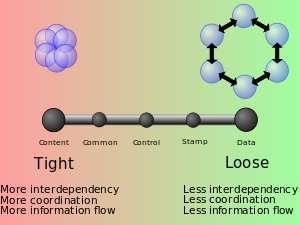
\includegraphics[scale=0.5]{CoupledLoose.png}
	\captionof{figure}{Tight and Loose Coupled systems\cite{wikitight}}\label{looseimage}
\endgroup

\subsection{Data flow and main agents}
\label{dataflow}

In a general Offloading Framework three components can be correctly identified: the device that needs to offload its work, the communication channel and the the device that helps boost performance and receives the work to be offloaded.
%\TODO Name the ofloadee and the ofloaded

The system proposed in this paper uses for communication a low power consumption implementation of the Bluetooth technology, called Bluetooth Low Energy \cite{BLE2}. This technology permits a high throughput of data to be transferred wireless with relatively low energy consumption over short distances ( below 10 meters ). The benefit the BLE communication brings is that the channel used has a very low impact on the system itself \cite{BLE}, but it has an innate drawback in the fact that it has a short range.

In order to mitigate this drawback, in this framework the device that provides the processing power is a small System on a Chip device that can either lend its power to mobile devices or act a gateway to other more powerful systems. The benefits for adding an intermediary for offloading solutions is that it keeps the simple goal of preserving battery power on the mobile device. The SoC is a small computer, without a battery that can be positioned almost anywhere: in a home, public transportation stations or work environments. By offering the possibility to access different processing power nodes would significantly reduce the mobile devices battery consumption.

Moreover, the implementation of the system permits interchangeability between the client and server devices. As such, if a device permits it, it can act as a server for another device, and thus managing to share some of the resources. The model proposed here will assume that the client is a mobile device based on the Android OS, while the server is a SoC, specifically a RaspberryPI (An ARM GNU/Linux box for \$25).

In a first stage, when a piece of code that can be offloaded is detected, the client device will scan for potential offloading nodes. If such a node is detected, it will try to connect and create a network between the two devices. Once the connection is established, the client will send it's offloading request, through either of the aforementioned methods. The server will respond with either request acknowledge or busy.

The server can accept a number of connections and requests per time frame, in order to not burden itself and thus becoming a bottle neck for the system as a whole. Once the request has been acknowledged and processed, the results will be sent back to the mobile device, depending on the offload method that is used. An exemplification of this data flow can be view in figure \ref{btoffload}.

\pagebreak

%show a picture here
\begingroup
	\centering
	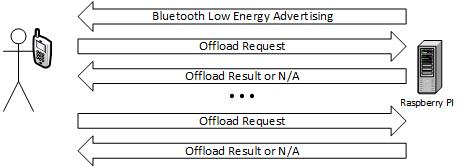
\includegraphics[scale=0.6]{BTOffloadArch.jpg}
	\captionof{figure}{Data flow architecture}\label{btoffload}
\endgroup

\section{Framework Definition and Implementation}
\label{implementation}

In order to achieve the desired performance and low energy consumption, an offloading software framework is proposed. The BLE Offloading Framework is structured as a client-server architecture that uses Bluetooth Low Energy technology in order to communicate.

\subsection{The client - Android Framework}

The BLEOffloadingFramework offers an Application Programmable Interface (API) for developers of applications on Android devices. Using the Bluetooth Low Energy framework available since Android version 4.2 these devices can scan and connect to other devices, without an impact on performance or power consumption.

At the current state of the project the framework represents a test application that connects through BLE to the server side program and sends small packets of data that mimics data transfer over a period of time.

%The offloading system is designed to offer methods through which a developer can register certain methods to be offloaded through RPC/RMI ( in which the application waits for a certain output ) or through the Loose coupling method ( where the application will be notified when results are available ). The users must select the desired method when first designing the application, but theoretical results show that a combination between the two methods seems to offer the best performance: perform an RPC call to the offload node on a separate thread and wait for the results in parallel to other tasks. BLEOffloadingFramework will offer methods and callbacks written in the Java programming language in order to simplify the task of offloading methods.

%In the loose coupling scenario, the developer creates a serializable class structure, by inheriting a class from the framework or implementing an interface and annotate methods of that class that can be offloaded. In this case, when the framework detects the right offloading conditions ( there is an offload node available and ready ) it will request and send that class through serialization to the server, which will perform the necessary calculations and return a result.

%Regarding the RPC/RMI method, the framework manages the methods that are marked for offloading and check if the offloading node is available and if it has that method available. In this case, the code is duplicated between client and server, but it has the added benefit of being faster, relative to the loose coupling method.

\subsection{The server - Linux Embedded System}

Because of the easy to use interface and availability of source code, the server is conceptualized on a Linux Operating System and uses the BlueZ\cite{BlueZ} open source Bluetooth stack. For connectivity, a Bluetooth 4.0 USB dongle is used. This permits a generality for the  system in the sense that it is not hardware specific - any Bluetooth chipset that abides to the standard can be used, even if it is directly embedded on the system, communicating through the UART interface, or through the USB protocol.

In order to facilitate development, the server is written in the C language. The basic server functionality is handling Bluetooth connections and responding in an efficient way to requests from clients as decided in the protocol mention in section \ref{dataflow}.

The server starts off by advertising its availability using BLE Advertising\cite{BLE2} in connectable mode. This permits clients to automatically connect to the server and create an L2CAP socket that becomes available for use in transmitting and receiving data. After a connection is established, the server application waits a predefined period of time for clients to send a request header, that contains the type of offloading and data type that the client expects to receive after the invocation of the methods.

%In case of the loose coupled system, the server will load a Java Virtual Machine and will pass the serialized object to it, perform the calculations and send the results. In case of the procedure calls, the server will detain a list of methods or functions that can be called and will execute them when the request is received.

%The server program is still a work in progress and the exact technologies and methodologies that will be used are to be determined after a series of performance tests.

\section{Testing Methodology}
\label{results}

In order to validate the offloading system, a series of performance and stress tests are the determining factor. In this chapter, the testing methodologies are described for the BLEOffloadFramework.

\subsection{Test setup}

In order to offer conclusive data, the test setup contains different types of mobile devices that can benefit from the Offloading Framework, in this case, two smart phone devices from different producers with different specifications. Both devices are using the Android Operating System, version 4.4, in order to benefit from the Bluetooth Low Energy technology.

Both devices are charged to maximum capacity, as indicated by the Android notification system and run the same applications. Example applications include simple programs that are computational intensive, such as image processing applications or route calculating algorithms, which are common algorithms among mobile devices.

The idea is to expose the device to a series of tests, conducted using UIAutomator, a testing tool for Android that emulates user behavior. The test sequence repeats a pattern of user touch inputs until the devices receives a low battery notification, after which the time it took for the device to deplete it's battery is measured as the time between the start of the UIAutomator test case and the low power event.

Several test cases are distinguishable: The case where offloading is disabled and when offloading is enabled using different methods. The results of these test cases will roughly predict the power consumption of the devices in real life scenarios and the initial data can be extrapolated in order to predict the overall gain of using the offloading system.

These tests should reveal that using the framework described in section \ref{architecture} will have an impact on energy consumption, in the sense that it takes a longer time to reach the low-battery notification. Exact empirical results will be available once the API for Android applications is completed.

\section{Conclusions}
\label{conclusions}

Consuming less energy has been a prime focus in mobile communities since the development of high end smart phone devices has exceeded the technological advancement of batteries.

Offloading computational intensive code from one device to another is a method through which power saving can be achieved and the BLEOffloadingFramework is one of many solutions available to handle this problem. This system offers a complete solution for Android application developers to bring new value to their programs and to receive more out of the mobile environment. The solutions presented here are scalable, designed to be easy to use and offer a new dimension when it comes to programming for the Internet Of Things.

Improvements to the system can also bring a new form of distributed performance boost, because, even though the case for a stable server and mobile client was discussed, the framework can be made to work with other mobile devices as well, permitting users to share their power between them in a seamlessly and easy way.


\end{multicols}

\begin{thebibliography}{1}

\bibitem{understandingBattery} Ferreira, Denzil, Anind K. Dey, and Vassilis Kostakos. {\em "Understanding human-smartphone concerns: a study of battery life." Pervasive computing.} Springer Berlin Heidelberg, 2011. 19-33.

\bibitem{batteryLife} Megan Geuss. {\em http://www.techhive.com/article/228189/SmartBat.html - Why Your Smartphone Battery Sucks}

\bibitem{Alex} Olteanu, Alexandru-Corneliu, Nicolae Tapus, and Alexandru Iosup. {\em "Extending the capabilities of mobile devices for online social applications through cloud offloading." Cluster, Cloud and Grid Computing (CCGrid), 2013 13th IEEE/ACM International Symposium on.} IEEE, 2013.

\bibitem{CloneCloud} Chun, Byung-Gon, et al. {\em "Clonecloud: elastic execution between mobile device and cloud." Proceedings of the sixth conference on Computer systems.} ACM, 2011.

\bibitem{Android} Developers, Android. {\em "What is Android."} 2011.

\bibitem{RPC} Srinivasan, Raj. {\em "RPC: Remote procedure call protocol specification version 2."} (1995).

\bibitem{wikitight} Coupling (computer programming) \url{http://en.wikipedia.org/wiki/Coupling_%28computer_programming%29}, Wikipedia

\bibitem{BLE2} Gomez, Carles, Joaquim Oller, and Josep Paradells. {\em "Overview and evaluation of bluetooth low energy: An emerging low-power wireless technology."} Sensors 12.9 (2012): 11734-11753.

\bibitem{BLE} Martelli, Flavia. {\em "BLUETOOTH LOW ENERGY."}

\bibitem{BlueZ} Krasnyansky, Maxim. {\em "BlueZ: Official linux bluetooth protocol stack."} (2003).

\end{thebibliography}

\end{document}
